


\section{Electromagnetic Calorimeter Cluster Finding}
%seed finding
%cluster building
It is observed that if a monopole traverses the barrel electromagnetic calorimeter (Ecal),
it leaves most of its kinetic energy in a single crystal and deposits smaller amounts
of ionisation energy in the neighboring crystals either down-stream or up-stream of the 
magnetic field for a monopole or anti-monopole respectively.  The up/down stream energy
deposits from the initial deposit arrive at later and later times reported by the Ecal 
crystals.  One expects little radiative energy associated with the Ecal signature.
Therefore, one can expect monopole energy deposits to appear as strips at constant $\phi$
of adjacent crystals in the Ecal where the energy profile is skewed either toward or 
away from the magnetic field.  One also expects the time signature in these strips to a 
skewness in the opposite direction.   

\begin{figure}[H]
\centering
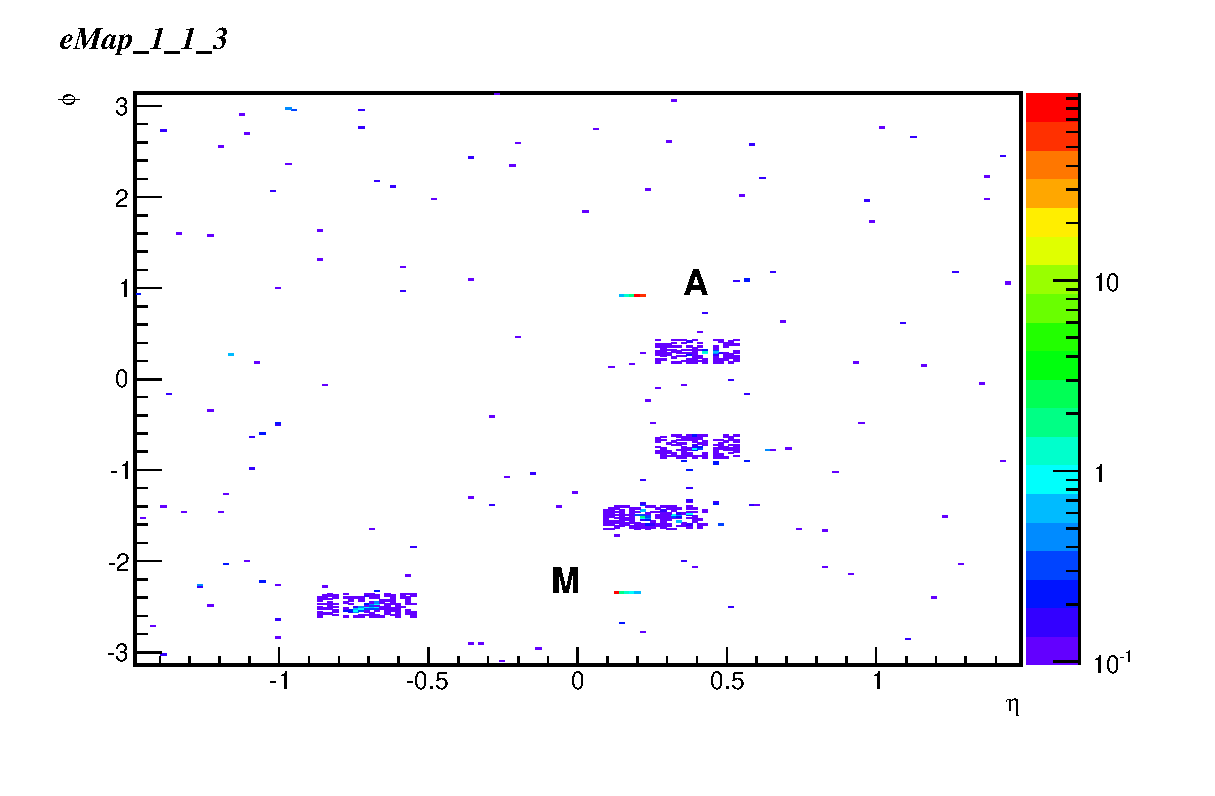
\includegraphics[width=0.75\textwidth]{plots/HiggsEcalMap_3.eps}
\caption{Typical energy flow of a monopoleis encountering the CMS electromagnetic
calorimeter in simulation.}
\label{fig:SimEcalMap}
\end{figure}

Seeds which consist of three Ecal crystals adjacent in the $\eta$ direction whose total
energy is above $50\;\mbox{GeV}$ are found by scanning through all possible such seeds in 
the Ecal.  When seeds overlap, the seeds are merged together.  Then all seeds are either
expanded or truncated such that their final length is 5 crystals.  If a seed is too short,
crystals are symmetrically added to either side of the seed (unless the seed is too close 
to the Ecal boundary).  If a seed is too long, the seed is truncated to the appropriate
length such that the maximum energy is found in the final seed. Finally, to each
seed two additional strips are added to either side of the seed.  This method produces a 
set of energy clusters consisting of 25 Ecal crystals in a 5x5 arrangement.

\begin{figure}[h]
\centering
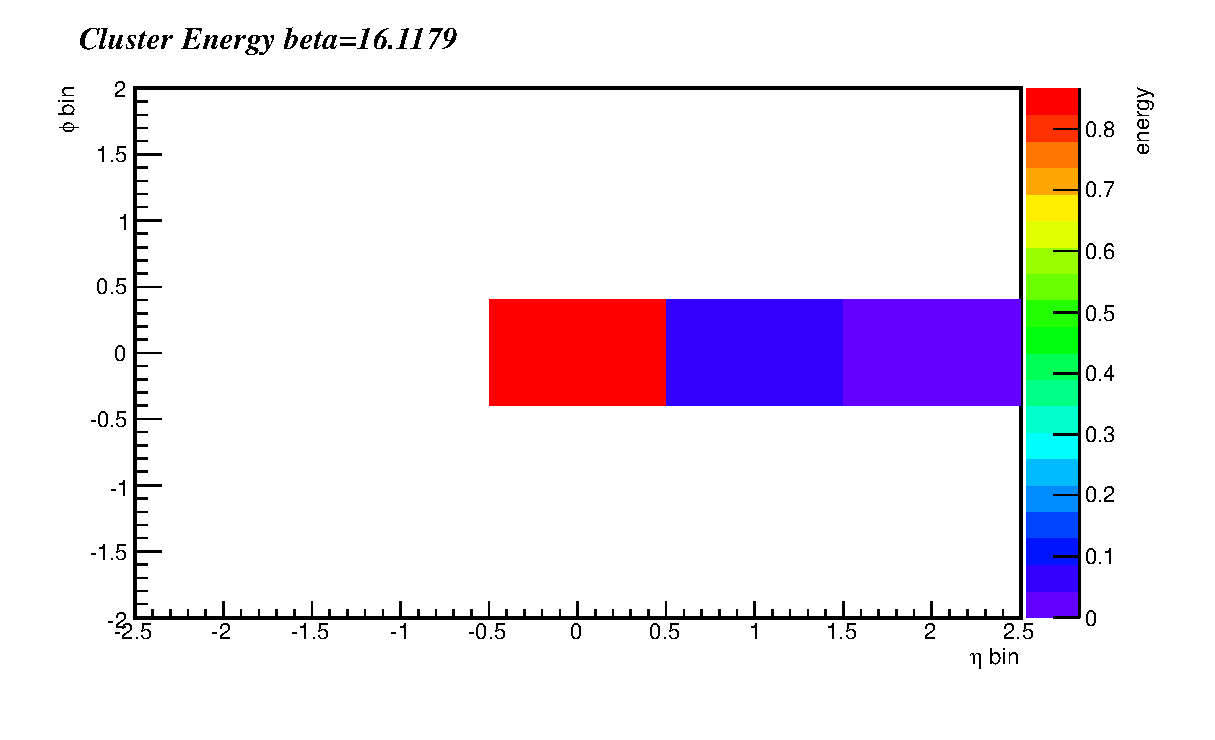
\includegraphics[width=0.75\textwidth]{plots/monoCluster.eps}
\caption{An example of a monopole cluster found in the CMS electromagnetic calorimeter.}
\label{fig:MonoCluster}
\end{figure}

A calibration technique is adapted to differentiate the clusters 
formed by a monopole encountering the Ecal.  The energy of each cell is normalized by 
total cluster energy, and each normalized cell energy is treated as a random variable.
The covariance matrix is formed for these random variables from a particle sample of clusters.
Then, the covariance matrix is inverted to form the concentration matrix.  
Now for each cluster a unique random variable may be calculated by following equation:
\begin{equation}
\beta = \sum_{i,j} (E_i-\bar{E}_i) H_{ij} (E_j-\bar{E}_j)\,,
\label{eq:beta}
\end{equation}
where $H_{ij}$ are elements of the concentration matrix.

